\documentclass[cjk,c,squeeze,shrink,dvipdfmx,12pt,handout]{beamer}
% 以下は決まり文句
\usepackage{bxdpx-beamer}                      % dvipdfmx用の fix
\usepackage{pxjahyper}                         % 日本語で'しおり'
\usepackage{minijs}                            % min10ヤダ
\usepackage{amsmath,amssymb,ulem}              % 数式、下線など。
\renewcommand{\kanjifamilydefault}{\gtdefault} % 既定をゴシック体に
% theme @see ./beamerthemeKansaiDebian.sty
\usetheme{KansaiDebian}
% Section 前に目次を挿入
\AtBeginSection[]{%
  \begin{frame}%
    <beamer>\frametitle{お品書き}%
    \tableofcontents[currentsection]%
  \end{frame}%
}%
% ---------------------------------------------------------
\title[Buster]{Debian 10 ``Buster''}
\subtitle[OSC 2019 Shimane]{%
  〜オープンソースカンファレンス 2019 Shimane〜%
}
\author[ささき]{%
  佐々木洋平/Youhei SASAKI\\[1em]
  \href{mailto:uwabami@debian.or.jp}{uwabami@debian.or.jp}
}
\institute[Debian JP Project]{%
  {\footnotesize{%
      Debian JP Project/関西Debian勉強会
    }}
}
\date[2019/09/27]{%
  {\footnotesize{2019年9月27日@松江テルサ}}
}
% ---------------------------------------------------------
\begin{document}
\setbeamercovered{transparent}
\takahashi[80]{ }
{%
  \setbeamertemplate{headline}{}
  \setbeamertemplate{footline}{}
  \begin{frame}
    \maketitle
  \end{frame}
}
% ---------------------------------------------------------
\begin{frame}[fragile]
  \frametitle{Disclaimer}
  \begin{itemize}
  \item 疑問、質問、ツッコミ、茶々、\alert{大歓迎}
  \item その場でインタラクティブにどうぞ
  \item ハッシュタグ: \alert{osc19sm}, \alert{\#debianjp} で
  \end{itemize}
\end{frame}
\begin{frame}{お品書き}
  \tableofcontents
\end{frame}
\section{Debianとは?}
% \takahashi[60]{Debianとは?}
% ---------------------------------------------------------
\begin{frame}[fragile]{Debian とは?}
  \alert{フリー/オープン}な\alert{ユニバーサル}オペレーティングシステムを
  作成しようとするボランティアベースのプロジェクト。
  \vfill
  \centering
  \begin{tabular}{|c|c|c|}
    \hline
    ディストリ          & 企業              & ボランティア      \\
    \hline
    Fedora              & RedHat支援あり    & あり              \\
    \hline
    RHEL                & RedHat            & なし              \\
    \hline
    CentOS              & RedHat支援あり    & あり              \\
    \hline
    \color{red}{Debian} & \color{red}{なし} & \color{red}{あり} \\
    \hline
    Ubuntu              & Canonical         & あり              \\
    \hline
    openSUSE            & SUSE支援あり      & あり              \\
    \hline
    SLES                & SUSE              & なし              \\
    \hline
  \end{tabular}
  \vfill
\end{frame}
% ---------------------------------------------------------
\begin{frame}[fragile]{Debian とは?}
  厳格/厳密なポリシーとガイドラインに沿った開発体制
  \begin{itemize}
  \item Debian 社会契約
  \item Debian フリーソフトウェアガイドライン
    \begin{itemize}
    \item オープンソースの定義の元
    \end{itemize}
  \item Debian Policy
  \end{itemize}
\end{frame}
% ---------------------------------------------------------
\begin{frame}[fragile]{Debian とは?}
  \begin{columns}
    \begin{column}{.58\paperwidth}
      \begin{itemize}
      \item
        Ubuntu や Raspbian といったディストリビューションのベースとなっている
      \item
        Debian Derivatives(Debian 派生ディストリビューション)との協力体制の整備
      \end{itemize}
    \end{column}
    \begin{column}{.4\paperwidth}
      \centering
      % https://upload.wikimedia.org/wikipedia/commons/thumb/6/69/DebianFamilyTree1210.svg/500px-DebianFamilyTree1210.svg.png
      % \includegraphics[height=.65\paperheight]{image201909/500px-DebianFamilyTree1210.png}
    \end{column}
  \end{columns}
\end{frame}
% ---------------------------------------------------------
\begin{frame}[fragile]{Debian とは?}
  世界規模で開発が行われており、63ヶ国、約1,100名のDebian公式開発者が開発
  を行っている。パッケージメンテナや翻訳などの貢献者も入れるともっと多く
  の開発者が参加していることになる。

  \begin{center}
    % \includegraphics[width=1cm]{image201909/debconf18_group.jpg}
    %
    % \includegraphics[height=0.4\paperheight]{image201909/debconf19_group.jpg}
  \end{center}
  % https://wiki.debconf.org/upload/thumb/4/43/Debconf18_group_photo_small.jpg/799px-Debconf18_group_photo_small.jpg
  % https://wiki.debian.org/DebConf/19/Photos?action=AttachFile&do=get&target=debconf19_group.jpg" -O debconf19_group.jpg
\end{frame}
% ---------------------------------------------------------
\begin{frame}[fragile]{Debian とは?}
  2019年9月の時点で、
  \pause
  \begin{itemize}[<+->]
  \item
    最新版は {\alert{Debian 10.1}}, ``Buster''
  \item
    提供パッケージ数は{\alert{約59,000}}
  \item
    公式にサポートするCPUアーキテクチャは{\alert{10}}
  \item {\alert{約2年毎}}にリリース
  \item next: Debian 11, ``Bullseye''
    \begin{itemize}
    \item %
      コードネームはトイ・ストーリーのキャラクターから
    \end{itemize}
  \end{itemize}
\end{frame}
% ---------------------------------------------------------
\begin{frame}[fragile]{Debian とは?: まとめ}
  \pause
  \begin{itemize}[<+->]
  \item Debianはフリー/オープンなOSを作成しようとするボランティアベースのプロジェクト。
  \item 自分たちの考えるフリーという言葉に関する定義、開発目的、パッケージングポリシーを厳格に決めている。
  \item 世界中に1,100人以上の開発者がおり、他のディストリビューションのベースとして採用されている。
  \item 約2年毎にリリースが行われ、多くのパッケージとアーキテクチャをサポートしている。
  \item 上記のような特徴から様々なところで利用されているディストリビューションである。
\end{itemize}
\end{frame}
%-----------------------
\takahashi[70]{そんな\\こんなで}
\takahashi[40]{Any Questions?}
%-----------------------
\section{Debian Updates: Buster}
%-----------------------
\takahashi[60]{Debian 10 ``Buster''}
{%
  \setbeamertemplate{headline}{}
  \setbeamertemplate{footline}{}
  \begin{frame}
    \centering
    % https://bits.debian.org/images/upcoming-buster.png
    % \includegraphics[height=\paperheight]{image201909/buster.png}
  \end{frame}
}
%-----------------------
\takahashi[60]{Debian 10 ``Buster'' \alert{Released!}}
%-----------------------
\begin{frame}[fragile]{Release Timetable}
  \framesubtitle{〜Debian 10 ``Buster'' Released!〜}
  \pause
  \begin{itemize}[<+->]
  \item 2014/11/09: Distribution codename announced
  \item 2017/06/17: Stretch is released, and buster becomes testing
  \item 2019/01/12: Transition freeze
  \item 2019/02/12: Soft freeze
  \item 2019/03/12: Full freeze
  \item 2019/07/06: Released!
  \item 2019/09/07: Updated Debian 10.1 released
  \end{itemize}
\end{frame}

\begin{frame}[fragile]{Artwork}
  \framesubtitle{〜Debian 10 ``Buster'' Released!〜}
  \begin{itemize}
  \item Alex Makas: futurePrototype
  \end{itemize}
  \begin{center}
    % 
\includegraphics[height=0.5\paperheight]{image201906/futurePrototype-wallpaper-1920x1080.png}
  \end{center}
\end{frame}

\begin{frame}[fragile]{Support Architectures}
  \framesubtitle{〜Debian 10 ``Buster'' Released!〜}
  \begin{itemize}
  \item amd64, i386
  \item arm64, armel, armhf
  \item mips64el, mipsel, mips
  \item ppc64el
  \item s390x
  \end{itemize}
\end{frame}

\begin{frame}[fragile]{Packages \& versions}
  \framesubtitle{〜Debian 10 ``Buster'' Released!〜}
  \begin{itemize}
  \item Linux 4.19 series
  \item GNOME 3.30, KDE Plasma 5.14, Cinnamon 3.8, MATE 1.20,\\
    Xfce 4.12, LXDE 0.99.2, LXQt 0.14
  \item Chromium 73.0, Firefox 60.7, Thunderbird 60.7.2
  \item LibreOffice 6.1, GIMP 2.10.8, Inkscape 0.92.4
  \item GNU Compiler Collection 7.4 and 8.3
  \item Perl 5.28, Python 3.7.2, Ruby 2.5.1, PHP 7.3, \\
    Golang 1.11, OpenJDK 11, Rustc 1.34
  \item MariaDB 10.3, PostgreSQL 11
  \item Emacs 26.1, Vim 8.1 \\
    etc.
  \end{itemize}
\end{frame}

\begin{frame}[fragile]{UEFI Secure Boot}
  \framesubtitle{〜Debian 10 ``Buster'': New Features〜}
  \begin{itemize}
  \item セキュアブートが有効な状態でもインストールと利用ができるようになった
  \item shim-signed, grub-efi-\{amd64,ia32\}-signed, Buster の Linux カーネルパッケージをインストールすれば既存の Debian でも利用可能
  \item DKMS が使用できないなど一部機能の制限あり
  \end{itemize}
\end{frame}

\begin{frame}[fragile]{AppArmorの有効化}
  \framesubtitle{〜Debian 10 ``Buster'': New Features〜}
  \begin{itemize}
  \item %
    多くのプロファイルは apparmor-profiles-extra をインストールすると利用可能
  \item %
    Linux カーネルパッケージで推奨 (Recommends) 依存設定
  \end{itemize}
\end{frame}

\begin{frame}[fragile]{nftables migration}
  \framesubtitle{〜Debian 10 ``Buster'': New Features〜}

  ネットワークフィルタリングの nftables への変更
  \begin{itemize}
  \item iptables コマンドは nftables を使用する iptables-nft がデフォルト
  \item 従来の iptables を使用するコマンドは iptables-legacy として提供
    \begin{itemize}
    \item %
      古いまま使いたい場合には
\begin{verbatim}
% sudo update-alternatives --config iptables
\end{verbatim}
      で\texttt{iptables-legacy}を選択(非推奨).
    \end{itemize}
  \item 他のディストリビューションでも同様に移行している
    \begin{itemize}
    \item %
      e.g. Red Hat Enterprise Linux 8.0
    \end{itemize}
  \end{itemize}
\end{frame}

\begin{frame}[fragile]{Wayland}
  \framesubtitle{〜Debian 10 ``Buster'': New Features〜}

  GNOMEのデフォルトは Wayland
  \begin{itemize}
  \item デフォルトで Wayland を使用
  \item Xorg はデフォルトでインストールされるので切り替えて使用可能
  \end{itemize}
\end{frame}

\begin{frame}[fragile]{usrMerge}
  \framesubtitle{〜Debian 10 ``Buster'': New Features〜}

  新規インストールは /usr Merge
  \begin{center}
    {\huge{%
        \begin{tabular}{lcl}
          \texttt{/bin}  & → & \texttt{/usr/bin}  \\
          \texttt{/sbin} & → & \texttt{/usr/sbin} \\
          \texttt{/lib}  & → & \texttt{/usr/lib}  \\
        \end{tabular}
      }}
  \end{center}

  \begin{itemize}
  \item Debian 以外から提供されるソフトウェアを利用している場合は要注意
  \item 既存のシステムでは \texttt{usrmerge} パッケージで移行可能
  \end{itemize}
\end{frame}

\begin{frame}[fragile]{misc.}
  \framesubtitle{〜Debian 10 ``Buster'': New Features〜}
  \pause
  \begin{itemize}[<+->]
  \item APTへのセキュリティ強化オプションの追加
  \item stable ポイントリリースに対する Unattended-upgrades の挙動
  \item ドイツ語話者用 man ページの飛躍的な改善
  \item Cryptsetup の on-disk LUKS2への変更
  \item CUPS 2.2.10 でのドライバーレス印刷機能
  \item Allwinner A64 ベースのデバイスでの基本機能サポート
  \item などなど
  \end{itemize}
\end{frame}

\begin{frame}[fragile]{Issues}
  \framesubtitle{〜Debian 10 ``Buster'': New Features〜}
  \pause
  \begin{itemize}[<+->]
  \item リリースノートの翻訳が未完
  \item glibc は Linux カーネル 3.2 以上を必要
  \item Wayland で一部アプリケーションが動作しない\\
    (synaptic, fcitx, アクセシビリティ機能)
  \item phpmyadmin, Redmine, VirtualBox などのパッケージは未収録
  \item Python2.7 は非推奨
  % \item More entropy
  \item OpenSSL のデフォルトが TLS 1.2 とセキュリティレベル 2
  \item ブラウザ, レンダリングエンジン, Go 関連のパッケージは制限付きのセキュリティサポート
  \item gnome-disk-utility: LUKS パスワード変更でデータ消失の危険性
    \\
    $\cdots$ などなど \hfill ⇒詳細はリリースノート参照のこと
  \end{itemize}
\end{frame}

\begin{frame}[fragile]{%
    Debian Updates: Stretch%
    \\[-.5em]{\normalsize{Debian 9.x: oldstable}}
  }
  \pause
  \begin{itemize}[<+->]
  \item 2017/06/17: Debian 9.0 released
  \item[] :
  \item 2019/01/23: Updated Debian 9.7 released
  \item 2019/02/16: Updated Debian 9.8 released
  \item 2019/04/27: Updated Debian 9.9 released
  \item[] :
  \item \alert{2019/07/06: Becomes oldstable} ← サポートはここから 1 年
  \item 2019/09/07: Updated Debian 9.10 released
  \end{itemize}
\end{frame}

\takahashi[70]{そんな\\こんなで}

\takahashi[40]{Any Questions?}

\section{日本語によるDebianの情報}

\begin{frame}[fragile]{日本語によるDebianの情報}
  \begin{itemize}
  \item Debian JP Project \\
    \url{https://www.debian.or.jp}
  \item 東京エリアDebian勉強会\\
    \url{https://tokyodebian.alioth.debian.org}
  \item 関西エリアDebian勉強会 \\
    \url{https://wiki.debian.org/KansaiDebianMeeting}
  \item Twitter \\
    \url{@debian_jp}
  \item slack:
    \url{debian-jp.slack.com}
  \end{itemize}
\end{frame}

\begin{frame}
  \frametitle{書籍情報}
  \begin{columns}
    \begin{column}{.5\paperwidth}
      \centering
      % http://image.gihyo.co.jp/assets/images/cover/2019/641908.jpg
      % \includegraphics[height=.6\paperheight]{image201909/sd2019.jpg}
    \end{column}
    \begin{column}{.5\paperwidth}
      \begin{itemize}
      \item %
        日本語での唯一の連載記事 \\
        「Debian Hot Topics」
      \end{itemize}
    \end{column}
  \end{columns}
\end{frame}

\begin{frame}
  \frametitle{書籍情報}
  \begin{columns}
    \begin{column}{.45\paperwidth}
      \centering
      % http://static.lulu.com/browse/product_thumbnail.php?productId=22625767&resolution=320
      % 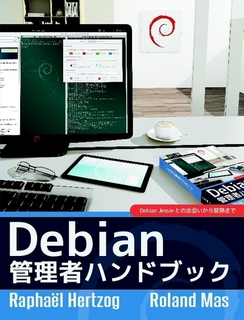
\includegraphics[height=.6\paperheight]{image201909/debianbook.jpg}
    \end{column}
    \begin{column}{.54\paperwidth}
      \begin{itemize}
      \item %
        英語書籍の翻訳版
        \begin{itemize}
        \item %
          原版: The Debian Administrator's Handbook
          \begin{itemize}
          \item %
            Rapha\"el Hertzog, Roland Mas
          \item \url{https://debian-handbook.info/}
          \end{itemize}
        \end{itemize}
      \item %
        日本語で読める(現状)唯一の書籍!
      \item %
        パッケージ版:
        \texttt{debian-handbook}
      \end{itemize}
    \end{column}
  \end{columns}
\end{frame}

% \takahashi[70]{そんな\\こんなで}

% \begin{frame}
%   \frametitle{今後のイベント}
%   \begin{itemize}
%   \item 8/17(土) 第177回東京エリアDebian勉強会
%     \begin{itemize}
%     \item \url{https://tokyodebian-team.pages.debian.net/2019-08.html}
%     \end{itemize}
%   \item 8/25(日) 第150関西Debian勉強会
%     \begin{itemize}
%     \item \url{https://wiki.debian.org/KansaiDebianMeeting/20190825}
%     \end{itemize}
%   \end{itemize}
% \end{frame}

\takahashi[40]{Any Questions?}
\takahashi[60]{Thanks!}

\end{document}
